\documentclass[urlcolor=blue,dvipsnames]{beamer}

\usepackage[utf8]{inputenc}
\usepackage{fancybox,fancyvrb}
\usepackage{environ,xspace,empheq}
\usepackage{tikz}
\hypersetup{colorlinks,linkcolor=,urlcolor=cyan}

\beamertemplatenavigationsymbolsempty
\setbeamertemplate{footline}[frame number]
\usetheme{Pittsburgh}

\newcommand\enumnum[1]{{\renewcommand{\insertenumlabel}{#1}%
      \usebeamertemplate{enumerate item} \,}}

\newcommand{\grad}{\nabla}
\newcommand{\ih}{\boldsymbol{\hat{\textbf{\i}}}}
\newcommand{\jh}{\boldsymbol{\hat{\textbf{\j}}}}
\newcommand{\vF}{\boldsymbol{\vec{\textbf{F}}}}
\newcommand{\Matlab}{\textsc{Matlab}\xspace}
\newcommand{\Octave}{\textsc{Octave}\xspace}


\title{9.1 Finding better numerical solutions \\ (than Euler's method)}

\subtitle{a lesson for MATH F302 Differential Equations}

\author{Ed Bueler, Dept.~of Mathematics and Statistics, UAF}

\date{\tiny \today}


\begin{document}
\setbeamertemplate{itemize item}{$\bullet$}
\setbeamertemplate{itemize subitem}{$\circ$}
\renewcommand{\thefootnote}{{\color{green} \arabic{footnote}}}

\begin{frame}
\titlepage

\centerline{\tiny for textbook: \, D. Zill, \emph{A First Course in Differential Equations with Modeling Applications}, 11th ed.}
%\color{green!40!blue}
\end{frame}


\begin{frame}{x}

\begin{itemize}
\item X
\end{itemize}
\end{frame}


\begin{frame}{see slides and video on Euler's method}

\begin{itemize}
\item \alert{see my \S 2.6 slides and video}
    \begin{itemize}
    \item you must understand everything in those slides!
    \end{itemize}
\item they showed this sequence for $\frac{dy}{dt} = t - y^2$, $y(0)=1$:

\bigskip

\hspace{-12mm} \mbox{
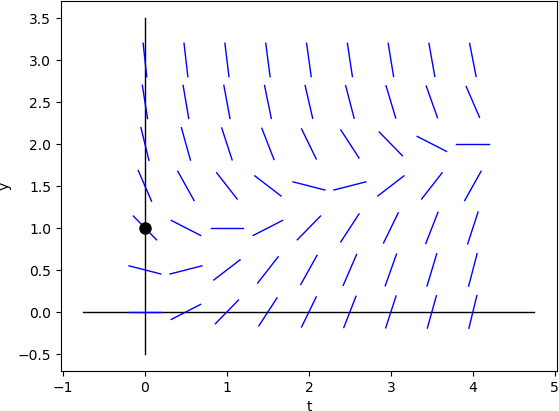
\includegraphics[width=0.31\textwidth]{figs/sequence-1} $\,$
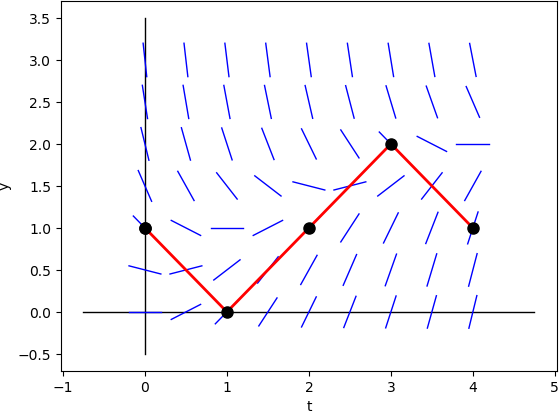
\includegraphics[width=0.31\textwidth]{figs/sequence-2} $\,$
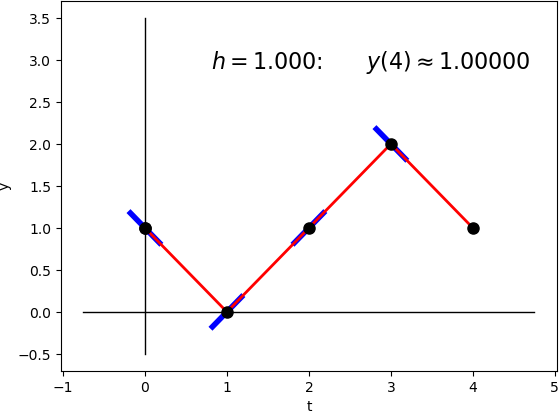
\includegraphics[width=0.31\textwidth]{figs/sequence-3} $\,$
}

\bigskip

\hspace{-12mm} \mbox{
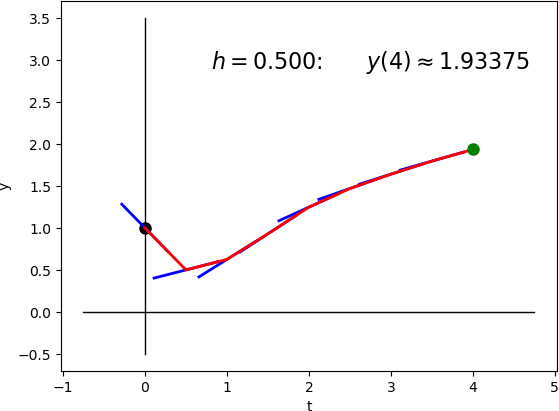
\includegraphics[width=0.31\textwidth]{figs/sequence-4} $\,$
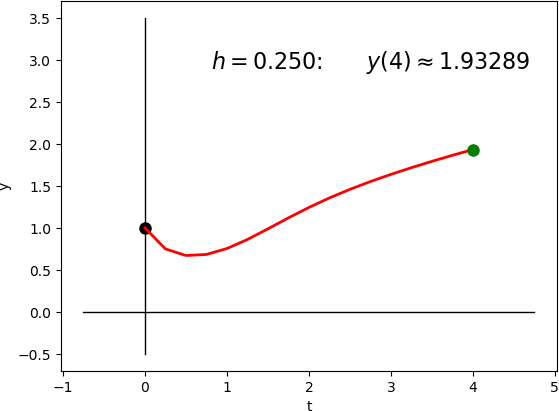
\includegraphics[width=0.31\textwidth]{figs/sequence-5} $\,$
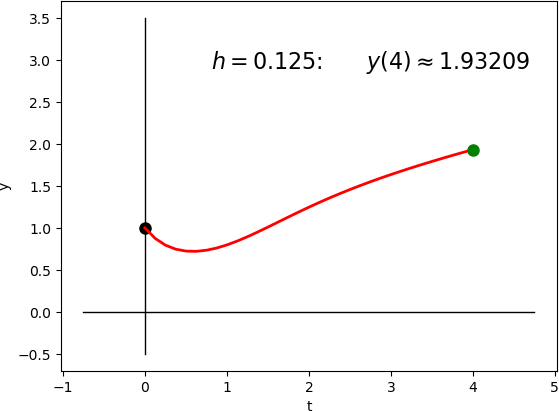
\includegraphics[width=0.31\textwidth]{figs/sequence-6}
}

    \begin{itemize}
    \item such a visualization must make sense!
    \end{itemize}
\end{itemize}
\end{frame}


\begin{frame}{x}

\begin{itemize}
\item X
\end{itemize}
\end{frame}

% for problem:
% >> f = @(t,y) t - y^2;
% >> optt = odeset('RelTol',RTOL,'AbsTol',1.0e-14);
% >> [tt,yy] = ode45(f,[0,4],1,optt); yy(end)
%ans =  1.93122683184240
%       -----------       <- 10 digits which agree for
%                            RTOL=1.0e-9,1.0e-10,1.0e-11,1.0e-12

% will use:  yexact = 1.9312268318427   based on above and RK4 with h=0.0001

% on same problem, for considering refinement:
% h=0.4, 0.2, 0.1, 0.05, 0.025

\begin{frame}{expectations}

\begin{itemize}
\item just watching this video is \emph{not} enough!
     \begin{itemize}
     \item see ``found online'' videos and stuff at

     \centerline{\href{https://bueler.github.io/math302/week10.html}{\tt \color{cyan} bueler.github.io/math302/week10.html}}
     \item \emph{read} section 9.1 in the textbook
     \item \emph{do} the WebAssign exercises for section 9.1
     \end{itemize}
\end{itemize}
\end{frame}

\end{document}

